\documentclass[UTF8]{article}
\usepackage[utf8]{inputenc}
\usepackage{ragged2e}
\usepackage[spanish]{babel}
\usepackage{anysize}
\marginsize{3cm}{3cm}{0.5cm}{3cm}
\usepackage{amsmath}
\usepackage{hyperref}
\usepackage{textcomp,gensymb}
\usepackage{float}
\usepackage{graphicx}
\usepackage{caption}
\usepackage{subcaption}
\usepackage{amsthm}
\usepackage{amssymb}
%\usepackage{unicode-math}
\usepackage{parskip}
\title{Propuesta de tésis}
%-----------------------------------------------------------------------------------------------------------------------------------------




\usepackage{float}



%\usepackage{sty/caption/subcaption}

\usepackage{multirow}
\usepackage[spanish]{babel}
\usepackage{caption}
%\usepackage{multicol}
%\usepackage{longtable}
%\usepackage{tabularx}

\usepackage{graphicx}
\usepackage{siunitx}

%%%%%%%%%%%%%%%%%%%%%%%%%%%%%%%%%%%%%%%%%%%%%%%%%%%%%%%%%%%%%%%%%%%%%%%%%%%%%%%%%%%%%%


\begin{document}
\begin{titlepage}
   \begin{center}
       \vspace*{1cm}
       \LARGE
       \textbf{Digitalización tridimensional por la técnica de luz estructurada para objetos con alta reflectividad}
 
       \vspace{0.5cm}
       
       \LARGE
        Placas de fijación para la recuperación ósea
 
       \vspace{1.5cm}
       \large
       \textbf{Estudiante : Daniel José Agudelo\\
       Director : Jaime Meneses Fonseca}
 
       \vfill
 
 
 
     
 
       
\includegraphics[width=0.4\textwidth]{Logo.png}
 
       Grupo de Investigación en óptica y tratamiento de señales (GOTS)\\
       Universidad Industrial de Santander\\
       Bucaramanga, Colombia\\
       \today
 
   \end{center}
\end{titlepage}



%-----------------------------------------------------------------------------------------------------------------------------------------
\newpage
\begin{abstract}
\end{abstract}
\medskip

%-----------------------------------------------------------------------------------------------------------------------------------------
\section{Introducción}

Pese a que el mundo que nos rodea en la cotidianidad es tridimensional, nuestra visión solo pueden acceder a él a través de imágenes bidimensionales. %¿cómo podríamos reconocer entonces la diferencia entre una esfera de un circulo?.

Se puede decir que nuestro cerebro necesita entonces datos adicionales en la imagen bidimensional para tener alguna percepción de la profundidad,el desarrollo humano más sobresaliente en este sentido fue la Estereopsis, la capacidad del cerebro de unir dos imágenes ligeramente diferentes para formar una sola con una sensación de profundidad.

%esto, junto con otros fenómenos como la sombra nos dieron la relación entre la naturaleza tridimensional del mundo y los cambios en la forma y color de un objeto en una imagen bidimensional, resolviendo así, la pregunta del párrafo anterior. 
\medskip

\begin{figure}[h]
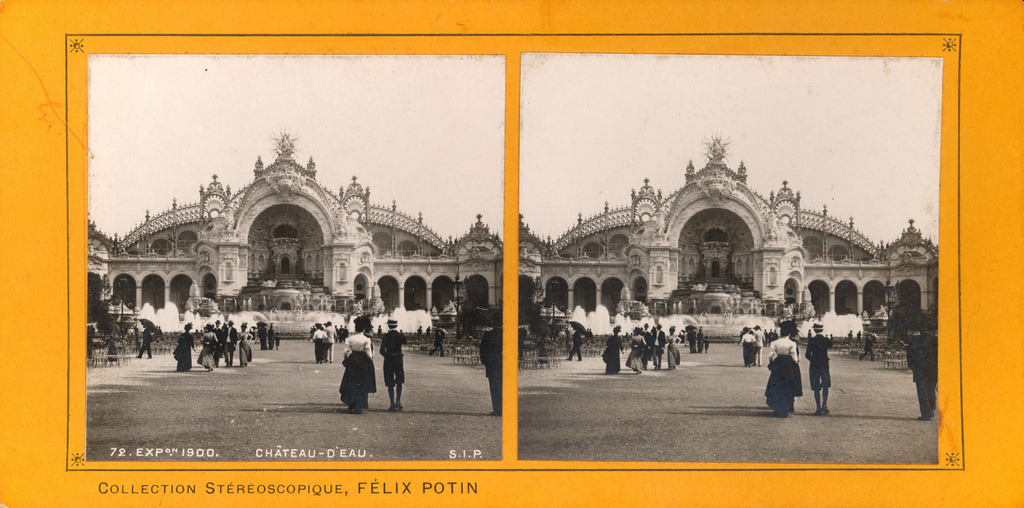
\includegraphics[width=10cm]{StereogramFrance.jpg}
\centering
\caption{Los estereogramas son dos imágenes tomadas desde posiciones ligeramente diferentes, utilizan la estereopsis, por lo que si se ve con un ojo cada una se percibirá profundidad en la imagen. \url{https://www.flickr.com/photos/photographic-heritage/15075096889}}
\label{im1}
\end{figure}


Pese a que nuestros ojos son muchas veces el sentido más valioso, tienen sus limitaciones, como parte de nuestro cuerpo  están sujetos a sufrir enfermedades y extenuarse, además de la dificultad para medir distancias con una precisión de milímetros. Se hace necesario, en el preámbulo de la era de la automatización, el enseñar a las máquinas a ver y medir las dimensiones de un objeto, a reconstruir un objeto.
%, usando para ello todos los métodos e instrumentos con los que contemos.

El instrumento óptico más cercano en cuanto a función de ojo es la cámara, que capta señales de intensidad y las ordena en una matriz bidimensional de píxeles, debido a esto último,la cámara, al igual que nuestros ojos, solo ve proyecciones bidimensionales del mundo tridimensional, hay una pérdida de información asociada a la distancia medida en dirección axial o del eje óptico de la cámara (eje z en ).

\begin{figure}[h!]
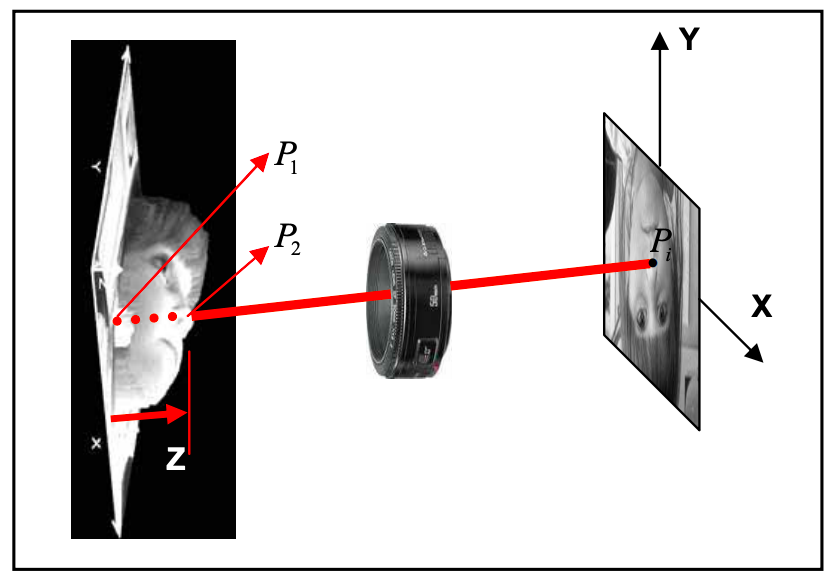
\includegraphics[width=10cm]{perdida3d.png}
\centering
\caption{imagen triangulación Ricardo Contreras []}
\label{im3}
\end{figure}
\medskip

Con base en la visión estereoscópica humana, los físicos e ingenieros han podido construir dispositivos de medida 3D que permite digitalizar la superficie de un objeto que se encuentre en el campo de visión de la cámara. Existen diferentes metodologías que permiten esto, de las cuales se destacan la visión estéreo, luz estructurada, e interferometría láser.
\medskip

La digitalización tridimensional "3DD" por sus siglas en inglés (3D digitalization) de un objeto se define como el almacenamiento dentro de una computadora o dispositivo digital de un conjunto de puntos que representen la información del contorno superficial del mismo. Es decir, que la superficie del objeto pueda representarse como una nube de puntos ubicados en un sistema de referencia tridimensional único que describe el mundo real.
%
%Una vez obtenida la nube de puntos puede ser confuso el visualizarla directamente en un dispositivo digital, dado que puede haber 
3DD tiene importantes aplicaciones en áreas de la sociedad que van desde la industria, donde se realiza control de calidad sobre objetos manufacturados[][], hasta la ciencia forense, donde se puede utilizar para encontrar modificaciones ilegales al número de placa de un automóvil[], también se puede hablar de aplicaciones a ramas mucho más modernas, como lo son el reconocimiento facial por parte de computadoras [] y la posibilidad de reproducir el objeto digitalizado bajo formatos CAD como el "STL" (Standard Triangle Language) gracias a las modernas impresoras 3D[], entre otros.
\medskip

%finalmente, dentro de estos métodos, el llamado método de proyección de franjas proyecta patrones que consisten 




%%%%%%%%%%%%%%%%%%%%%%%%%%%%%%%%%%%%%%%%%%%%%%%%%%%%%%%%%%%%%%%%%%%%%%%%%%%%





\section{Marco teórico}

%Como se ha mencionado,la digitalización tridimensional consiste en almacenar y reproducir correctamente un objeto del mundo real en una computadora o dispositivo digital, el dispositivo por excelencia que cumple con los propósitos de la visión humana es la cámara, y dado el símil entre estos últimos, la mayoría de metodologías buscan relacionar información adicional perteneciente a la imagen bidimensional captada para realizar la digitalización. 

\subsection{Modelo pinhole de la cámara digital}


En el grupo se ha trabajo con la estrategia de [] donde se utiliza el \textbf{modelo de pinhole} para la cámara y el proyector en procesos de calibración. Este es un modelo matemático que se basa únicamente en geometría para describir el proceso de formación de imagen como la proyección del objeto en el espacio tridimensional sobre un plano bidimensional.

\begin{figure}[h!]
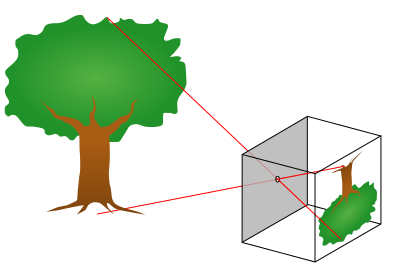
\includegraphics[width=8cm]{camera.png}
\centering
\caption{Esquema sencillo del modelo pinhole, el plano imagen generalmente se toma a una distancia $f$ antes del punto central garantizando que la imagen no se invierta.}
\label{im2}
\end{figure}
\medskip

Se definen los sistemas de referencia, para una cámara el punto en donde convergen los rayos se denomina punto central $C$ de la cámara, un segmento de recta de longitud $f$ conecta dicho punto con el punto central del llamado plano imagen llamado punto principal $O_{C}$, el segmento coincide con el eje óptico de la cámara.
%
Tanto el punto central $C$ de la cámara como el punto principal  del plano imagen definen los orígenes de los sistemas de referencia, el objeto ubicado en el espacio $\mathbb{R}^3$ está relacionado con el sistema de referencia de coordenadas cartesianas $\{X_{c},Y_{c},Z_{c}\}$ de la cámara mientras que la proyección de su imagen en $\mathbb{R}^2$ está relacionada con el sistema de referencia del arreglo bidimensional $\{u,v\}$ de píxeles de la cámara.
\medskip

\begin{equation}
 \{X_{c},Y_{c},Z_{c}\} \mapsto \{u,v\}     
\end{equation}
%
Se puede ver fácilmente la primera de las relaciones geométricas entre los dos sistemas de referencia, un punto $P$ en el espacio $\mathbb{R}^3$ se proyecta a través de una recta que atraviesa el arreglo en $\mathbb{R}^2$ de la cámara en el punto $p$ y llega al punto $C$, los triángulos  $\mathbf{CX_{c}Z_{c}}$ y $\mathbf{Cuf}$  así como  $\mathbf{CY_{c}Z_{c}}$ y  $\mathbf{Cvf}$ son semejantes de manera que:  
\medskip

\begin{equation}
\frac{X_{c}}{u} = \frac{Z_{c}}{f} \quad \wedge \quad \frac{Y_{c}}{v} = \frac{Z_{c}}{f}    
\end{equation}
%
La relación se completa utilizando la geometría proyectiva, en la cual se define la matriz homográfica \textbf{A} de dimensiones 4$\cdot$3 que garantiza la siguiente ecuación:

\begin{equation}
 ( fX_{c},fY_{c},Z_{c})^T  = \mathbf{A}  (X_{c},Y_{c},Z_{c},1)^T,
\end{equation}
%
se encuentra por inspección, que 

\begin{equation}
 \mathbf{A}   = \left( \begin{array}{cccc}
f & 0 & 0 & 0\\
0 & f & 0 & 0\\
0 & 0 & 1 & 0\end{array} \right) 
\end{equation}
%y se definen así; los planos donde se está generando la imagen llamado plano virtual y el plano real o plano del mundo, situado en la CCD 

Añadamos además que el arreglo bidimensional de píxeles no es un espacio discreto si no que se aproxima a un espacio continuo con un factor de conversión generalmente calculado en unidades de píxel/mm y que, además el origen de coordenadas del arreglo puede no coincidir con el punto $O_{c}$ se puede comprobar que :
\medskip

\begin{equation}
 \mathbf{A}   = \left( \begin{array}{cccc}
m_{x}f & 0 & x_{0} & 0\\
0 & m_{y}f & y_{0} & 0\\
0 & 0 & 1 & 0\end{array} \right) 
\end{equation}

%
Donde $m_{x}$ y $m_{y}$ son los factores de conversión ( de forma general se toman como diferentes ) y el punto $(x_{0},y_{0})$ es el origen del sistema bidimensional definido en milímetros, el modelo se completa añadiendo factores en la matriz $\textbf{A}$ que corrijan aberraciones en la lente de la cámara, la combinación de factores en dicha matriz es conocida como parámetros intrínseco de la cámara.

%
A menudo se añade un tercer sistema de referencia conocido como sistema del mundo, ubicado fuera del punto $C$, cuyas coordenadas cartesianas en el espacio tridimensional $\{X_{w},Y_{w},Z_{w}\}$ se relacionan con las del sistema de referencia centrado en $C$. como todo par de sistemas de referencia en el espacio,por una matriz de rotación y una de traslación de la siguiente manera:
\medskip

\begin{align}
  \{X_{c},Y_{c},Z_{c}\} &\mapsto   \{X_{w},Y_{w},Z_{w}\}  \quad \Rightarrow \\
     (X_{c},Y_{c},Z_{c})^T  &= \mathbf{R} (X_{w},Y_{w},Z_{w})^T- \mathbf{R} (X_{w0},Y_{w0},Z_{w0})^T
\end{align}

%
Donde el la matriz \textbf{R} es una matriz de rotación y $(X_{0},Y_{0},Z_{0})^T$ son las coordenadas del origen del sistema centrado en $C$ medidas respecto al sistema del mundo.

%
De la misma manera que el caso anterior, debemos expresar estas matrices de transformación y vectores en sus versiones homográficas : 
\medskip

\begin{equation}
     (X_{c},Y_{c},Z_{c},1)^T  = \mathbf{B} (X_{w},Y_{w},Z_{w},1)^T ,
\end{equation}
Donde \textbf{B} será :

\begin{equation}
    \mathbf{B}   = \left( \begin{array}{cc}
R & -RP_{w0}\\
0 & 1\end{array} \right), \quad \vec{P_{w0}} = (X_{w0},Y_{w0},Z_{w0})^T.
\end{equation}

%
Los factores que componen la matriz \textbf{B} se conocen como parámetros extrínsecos de la cámara.  
%
Para el proyector se utiliza el mismo modelo de pinhole,en teoría la única diferencia radica en que los rayos de luz salen desde el punto central del proyector en vez de entrar a él [].
\medskip
%%%%%%%%%%%%%%%%%%%%%%%%%%%%%%%%%%%%%%%%%%%%

\subsection{Digitalización 3D por vía óptica}




%
De las diferentes metodologías que permiten la 3DD de objetos,los criterios clave que definen su eficiencia son la resolución y el tiempo de procesamiento de datos. Las llamadas metodologías no invasivas se realizan sin contacto directo con el objeto a reconstruir, lo cual garantiza que no se afecte en el proceso. Dentro de estas estrategias no invasivas, las metodologías ópticas se clasifican en pasivas y activas. A pesar de que en su mayoría utilizan cámaras como dispositivos para capturar imágenes, las primeras no requieren una fuente controlada para iluminar la superficie del objeto, mientras las segundas necesitan si lo requieren con frecuencia.
\medskip

El principio básico por el que se codifica la información axial se basa en la triangulación, un esquema sencillo que ilustra este principio es el siguiente:
\medskip

Asumiendo ausencia de aberraciones en los instrumentos ópticos y el régimen de la óptica geométrica el rayo $\overline{O_{2}A}$ es controlado e identificable en la imagen de la cámara. El plano PR define la superficie de focalización de los dispositivos situados en $O_{1}$ y $O_{2}$, generalmente, uno de ellos será un detector y el otro una fuente. Cuando no se encuentra el objeto en el rango de visión del detector el rayo  $\overline{O_{2}A}$ intercepta PR en A y es focalizado en A', cuando el objeto está presente el objeto se intercepta en P y es focalizado en B'.
\medskip

El cálculo de la coordenada Z medida respecto a O' se basa enteramente en las relaciones de los triángulos $O_{1}O_{2}P$ y $ABP$ de manera que : 
\medskip


\begin{equation}
\frac{D}{L-Z} = \frac{\overline{AB}}{Z}  
\end{equation}
%
Los parámetros D y L del sistema se toman como fijos y conocidos con precisión. siendo la única incógnita encontrar la longitud del segmento $\overline{AB}$. Los puntos A' y B' sobre el plano de imagen de la cámara se relacionan linealmente con su contraparte en el plano PR.
\begin{equation}
\overline{AB} = m\cdot\overline{A'B'}  
\end{equation}
\medskip

Donde m se conoce como factor de ampliación transversal de la lente de la cámara, finalmente reemplazando : 
\begin{equation}
Z = \frac{L\cdot\overline{A'B'}}{D/m+\overline{A'B'}}
\end{equation}
\medskip

El punto crucial en el desarrollo consiste en identificar adecuadamente los puntos A' y B' y del tratamiento digital que permite esto se clasifican los diferentes métodos. Por ejemplo, si se tratara de triangulación láser se debe calcular el centro del spot láser en la imagen, mientras que si es visión estéreo se deben calcular en cada imagen la posición del mismo punto de la superficie del cuerpo.

%Dado que en su mayoría los métodos ópticos metrológicos utilizan este principio, la clasificación de los mismo depende de la manera en que se codifique la información que permita realizar la correspondencia, a continuación algunos de los métodos más conocidos:
\medskip



\subsection{Métodos ópticos pasivos}

\subsubsection{Visión estéreo}

El método de visión estéreo proporciona la digitalización tridimensional comparando dos imágenes del mismo objeto a través de dos cámaras a diferentes perspectivas, similar a la Estereopsis. A partir de la correcta calibración de los sistemas se pueden encontrar las coordenadas del objeto una vez identificado el punto del objeto en los píxeles de las dos cámaras.

El desempeño del método es altamente dependiente del modelo usado para establecer la correspondencia entre los píxeles. Objetos que no poseen mucha textura o información superficial característica generan inconvenientes en la búsqueda de puntos correspondientes. 
\medskip

\subsubsection{Profundidad por desenfoque}

Debido a la profundidad de campo de visión limitado de la cámara sobre la imagen aparecerán puntos del objeto 3D focalizados y otros borrosos. Encontrando un criterio matemático para determinar qué puntos de la escena están focalizados se puede generar un desplazamiento relativo entre objeto y cámara para barrer toda la superficie. Con el criterio y el desplazamiento se puede digitalizar la superifice del objeto. El desplazamiento relativo se puede realizar moviendo el objeto, la cámara, o variando la focalización de ésta última.
%El método consiste en encontrar una relación entre dos imágenes de la misma escena enfocadas en puntos diferentes, relacionando las dos imágenes, generalmente una desenfocada y la otra no, es posible encontrar una relación para las coordenadas 3D del objeto.
%
%Este método no utiliza dos cámaras capturando el mismo instante, si no más bien, una cámara capturando dos, por ello es difícil implementarla para digitalizaciones en tiempo real.
\medskip


\subsection{Métodos ópticos activos}

\subsubsection{Triangulación láser}

Un haz de luz proveniente de un láser incide oblicuamente sobre un objeto; posteriormente una cámara captura la imagen, se observa el spot láser que intercepta el punto sobre la superficie del objeto. Para digitalizar la superficie del objeto se desplaza el haz láser, puede ser proyectado un conjunto de puntos con espaciado uniforme o una franja que se desplaza.
%puede ser proyectado un arreglo de puntos con un espaciado uniforme o una sola franja.la información se codifica en el corrimiento de los puntos o de la franja proyectadas.

Las desventajas del método consisten en que el escaneo del láser se realiza desplazando los puntos o la línea por toda la superficie, por ende es un método lento,  presenta el ruido Speckle típico en sistemas de luz altamente coherente.
\medskip


\subsubsection{Tiempo de vuelo}

Similar al uso por parte de aves o murciélagos del sonar, el método del tiempo de vuelo envía una señal, se registra el tiempo en que la señal parte de la fuente y regresa a la cámara o sensor. la distancia de la fuente a cualquier punto de la superficie puede ser recuperada en base al tiempo medido y la velocidad de la luz, generalmente, y dado las dificultades que surgen al medir tiempos tan pequeños, la señal enviada es generalmente modulada con patrones sinusoidales de frecuencias de alrededor de 20 Mhz. genralmente se usa luz láser debido a la direccionalidad de la misma.
\medskip

Las desventajas vienen de la baja resolución dada por la dificultad de muestrear la señal de alta frecuencia requerida por el valor tan alto de la velocidad de la luz. \medskip




\subsubsection{Interferometría láser}


Como se sabe desde la óptica física, dos o más ondas electromagnéticas coherentes pueden ser superpuestas en un solo punto, el llamado fenómeno de interferencia encuentra su ejemplo más útil al utilizar frentes de onda planos. se encuentran máximos o mínimos a lo largo del espacio dependiendo de la diferencia de fase entre los frentes y por ende, de la diferencia entre el camino óptico del mismo.
\medskip

la generación de franjas de interferencia evidencia la presencia de caminos ópticos entre puntos de la superficie del objeto. La diferencia de fase en las franjas codifica dicha distancia. Recuperando la fase se obtiene la topografía del objeto.
%Se componen principalmente de una fuente láser, una cámara y elementos ópticos como espejos o divisores de haces que imponen las diferencias de camino óptico.
\medskip

Las ventajas de este método es su resolución, del orden de la longitud de onda del láser utilizado, las desventajas son su elevada sensibilidad vibraciones externas al montaje, desencadenante de ruido en la señal capturada.
\medskip
%Los diferentes interferómetros se diferencian por la forma en la que imponen estas diferencias de caminos ópticos entre los dos haces,en el interferómetro de Youg por ejemplo, se hace incidir un solo frente de onda normalmente sobre una superficie con dos ranuras 
\subsubsection{Proyección de franjas}

El método de proyección de franjas "FPP" (Fringe projection profilometry) hereda el principio básico de la interferometría láser, la información es codificada en una diferencia de fase de un patrón sinusoidal proyectado respecto a un plano de referencia, sin embargo, la proyección del patrón se realiza por medio de un sistema de proyección de video (video proyector).

Al depender de la medida de la fase, es robusto frente a la iluminación externa, y al utilizar un video-proyector como fuente de iluminación es menos sensible frente a las vibraciones externas, permite la digitalización simultánea del campo entero de la cámara.
%Dentro de los métodos de luz estructurada aquellos que utilizan patrones periódicos ,por ejemplo, funciones sinusoidales se destacan por su versatilidad y por ser robustos ante el ruido del ambiente, el método de proyección de franjas es una variante del método de triangulación láser, que utiliza el principio mencionado previamente, 

El FPP ha sido el protagonista gracias a sus ventajas mencionadas previamente, por esto, es un método con el que se ha trabajado en numerosos proyectos del GOTS [][][] y con el que se trabajará el presente, la siguiente subsección profundiza en el método:

\subsection{Proyección de Franjas}



El FPP utiliza un montaje esquematizado en \ref{im1}. 
\medskip

\begin{figure}[h!]
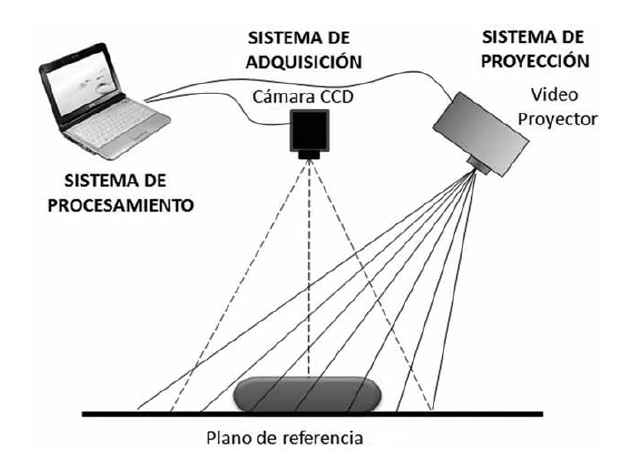
\includegraphics[width=10cm]{Montaje1.png}
\centering
\caption{Esquema del equipo utilizado en el método de proyección de franjas, esquema tomado de [].}
\label{im1}
\end{figure}


El video proyector ilumina el objeto a reconstruir con patrones de intensidad generados desde una computadora,la cámara captura las imágenes del objeto donde se encontrará una propiedad en donde se codifica la topografía del objeto, en este caso, un cambio en la fase.
\medskip


El método se divide en 4 etapas representadas en el siguiente esquema :

\begin{figure}[h!]
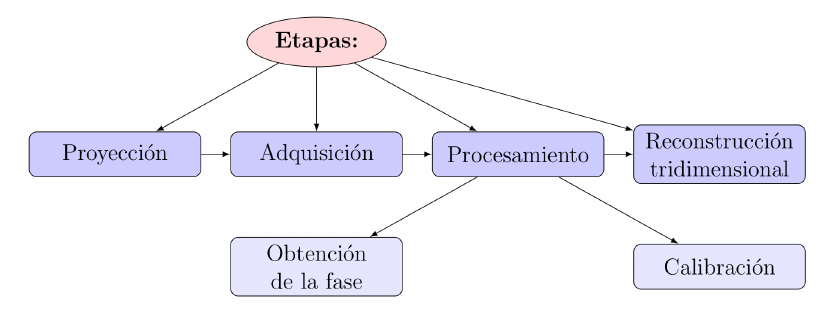
\includegraphics[width=12cm]{Esquema1.png}
\centering
\caption{Etapas del método de proyección de franjas, esquema tomado de []}
\label{im2}
\end{figure}


\subsubsection{Proyección}

Se genera una imagen a través de cualquier software, en este caso se trabajará con MATLAB por su facilidad para controlar la señal de video del proyector y cámara gracias a su lenguaje estructurado, por su tratamiento matricial de datos y por los resultados en trabajos anteriores en el grupo.La imagen proyectada obedece a una intensidad distribuida en un arreglo bidimensional m$\cdot$n donde m y n serán números enteros que cubren la resolución total de la matriz de sensores del proyector (cantidad de píxeles en dirección horizontal y vertical).
\medskip


Para este caso se genera la imagen con una función sinusoidal, las variables se eligen de manera que la forma proyectada sea de franjas paralelas horizontales o verticales, la forma básica usada en el software será :

\begin{equation}
    I(m,n) = A + B\cdot cos  \left( \frac{2\pi m}{p}\right),
    \label{eq1}
\end{equation}

el valor p define un paso o separación entre dos franjas consecutivas en píxeles, una frecuencia espacial. Los valores de las constantes A y B se definen tanto para evitar valores negativos incoherentes con la definición de intensidad como para permitir el máximo contraste, usualmente :
\medskip
%$m,n$} serán las coordenadas en la matriz bidimensional del computador desde el cual proyecta el video proyector.
\begin{equation}
A = B = \frac{1}{2}.    
\end{equation}
%Se realiza un script en MATLAB con el objetivo de generar una imagen, que no es más que una matriz de dimensiones x*y donde x y y serán números enteros que van desde 1 hasta s-1, con s la resolución de la pantalla ( cantidad de píxeles en dirección vertical u horizontal ), la función tendrá a la variable independiente x si se desean franjas horizontales o y si se desean verticales, así : 

\subsubsection{Adquisición}

En esta etapa una cámara CCD es utilizada para capturar imágenes  monocromáticas del objeto,si primero tenemos la imagen de un plano de referencia PR sabemos que la fase tendrá aproximadamente una relación lineal, de modo que la variación de fase lineal obtenida posteriormente por la presencia del objeto  puede traducirse a coordenadas en $Z_{w}$, relativas al plano PR.Las intensidades para el plano PR y en presencia del objeto capturadas por la cámara se plantean como:
\medskip



\begin{align}
    I(u,v) &= I_{0}(u,v) + I_{C}(u,v)\cdot cos\left( \frac{2\pi u}{p_{0}}\right) ,
    \\
    I(u,v) &= I_{0}(u,v) + I_{C}(u,v)\cdot cos\left( \frac{2\pi u}{p_{0}}+ \Delta\phi(u,v)\right).
    \label{eq2}
\end{align}
Donde la función $I_{0}$ es la intensidad captada causada por fuentes ajenas al proyector, $I_{C}$ la intensidad de contraste y $\Delta\phi$ será la diferencia de fase con respecto a la fase del plano de referencia [] y las coordenadas ($u$,$v$) serán las componentes horizontal y vertical en el arreglo bidimensional de píxeles en la cámara. Nótese que al realizar la resta entre las fases de la imagen con el objeto y en el plano PR se eliminan las distoriciones no lineales iniciales en las franjas causadas por distorciones en las lentes y proyección no telecéntrica.
\medskip
\subsubsection{Procesamiento}


Las ecuaciones 1.15 y 1.16 tienen la forma I=$A+Bcos(\phi)$, donde $A$, $B$ y $\phi$ son incógnitas e $I$ es una matriz que posee información de las variaciones de intensidad y corresponde a los datos de entrada. El problema consiste en realizar un procesamiento digital que me permita calcular las incógnitas a partir de los datos de entrada para cada píxel en el arreglo de sensores de la cámara.
%Llegado a esta etapa el paso a seguir consiste en realizar la completa \textbf{calibración} del sistema CCD-Objeto-Proyector, la calibración consiste en el proceso que permite encontrar la relación entre las coordenadas de la imagen bidimensional de la cámara y de la pantalla líquida del video-beam con un sistema de coordenadas tridimensional usualmente centrado en el objeto, para posteriormente encontrar la relación entre la fase deformada con la profundidad.
\medskip

%; es decir, encontrar la matriz de transformación que me relacione vectores de posición para los sistemas de referencia utilizados.
%En el grupo se ha trabajo con la estrategia de [] donde se utiliza 
%el \textbf{modelo de pinhole} para la cámara y el proyector. El esquema del modelo de pinhole utilizado para la cámara es el siguiente:
El propósito del proceso de calibración es el de relacionar la diferencia de fase con la coordenada $Z_{w}$ medida respecto al plano de referencia PR.  Existen métodos analíticos que hacen uso del mencionado modelo del pinhole. Se encuentran los elementos matriciales que describen los parámetros extrínsecos e intrínsecos de los dos instrumentos, y gracias a esto se realiza la conversión fase altura. Diferentes metodologías elaboradas el en grupo pueden utilizarse [][].
\medskip

Sin embargo existe una alternativa experimental relativamente sencilla, el principio consiste en relacionar la diferencia de fase directamente con la profundidad $Z_{w}$, mediante un ajuste polinomial, en este caso : 
\medskip

\begin{equation}
    Z_{w} = X_{1}\Delta\phi(u,v)^2 + X_{2}\Delta\phi(u,v)+ X_{3},
\end{equation}
donde los tres coeficientes $X_{i}$ con $i=1,2,3$ son constantes que deben ser calculados para cada píxel, el proceso experimental consiste en utilizar un tablero plano con una cubierta blanca opaca, colocarlo de manera que su vector normal sea colineal al eje óptico de la cámara, proyectar y obtener la fase mediante los métodos explicados a continuación y repetir este procedimiento a lo largo de un volumen de calibración.
\medskip

El volumen se define moviendo mediante un tornillo de precisión el tablero plano a pasos de $\Delta Z_{w}$ conocidos a lo largo de un intervalo $\{-Z_{wmax},Z_{wmax}\}$. Al centro de dicho intervalo se le asigna $\phi_{0}$ y para este valor $Z_{w}=0$.
%matrices con los factores extrínsecos e intrínsecos de la cámara y el proyector, aunque usualmente el sistema de referencia del mundo se hace coincidir con el sistema de referencia fijo en la pantalla líquida del proyector. Diferentes metodologías para realizar esto serán descritas en la sección de metodología.
\medskip

Posterior al proceso de calibración se realiza el proceso de cálculo de la fase, de las diferentes metodologías usadas para obtener el valor punto a punto de esta función de diferencia de fase se utiliza el método de corrimiento de fase ( "phase shifting" ), se introducen en \ref{eq1} diferentes desfases adicionales de $\theta_{i}$,dado que se necesitan ecuaciones linealmente independientes,el intervalo que se subdivide es $(0,2\pi]$ y dado que se tienen tres incógnitas en \ref{eq2}, se necesitan al menos 3 subdivisiones $\theta_{i}=\frac{2\pi}{3},\frac{4\pi}{3},2\pi$ que darán 3 ecuaciones linealmente independientes con las cuales se resolverá el sistema para $I_{0}$, $I_{m}$ y $\Delta_{\phi}$, para este caso tenemos desde \ref{eq1}:
\medskip

\begin{eqnarray}
 I_{1}(m,n) = I_{0}(m,n) + I_{C}(m,n)\cdot cos\left( \frac{2\pi m}{p}+ \Delta_{\phi}(m,n)+\frac{2\pi}{3}\right)
 \\
 I_{2}(m,n) = I_{0}(m,n) + I_{C}(m,n)\cdot cos\left( \frac{2\pi m}{p}+ \Delta_{\phi}(m,n)+\frac{4\pi}{3}\right)
 \\
 I_{3}(m,n) = I_{0}(m,n) + I_{C}(m,n)\cdot cos\left( \frac{2\pi m}{p}+ \Delta_{\phi}(m,n)+2\pi\right)
\end{eqnarray}

Si ahora definimos :
\medskip

\begin{align}
I_{c} = I_{i}\cdot cos( \theta_{i}),
\\
I_{s} = I_{i}\cdot sen( \theta_{i}).
\end{align}
%
Podemos resolver el sistema, en base a la ortogonalidad de las funciones trigonométricas, la fase será : 
\medskip
\begin{equation}
\Delta_{\phi}(m,n) =tan^{-1}\left( \frac{\sum I_{s}}{\sum I_{c}}\right) 
\end{equation}

Sin embargo, esta fase está obtenida a partir de una función trigonométrica inversa, lo que hace que esté acotada por intervalos de $2\pi$, si pensamos en la fase absoluta como una función continua debemos entonces realizar un proceso de desenvolvimiento de fase.

\subsubsection{Desenvolvimiento de fase}

Básicamente lo que se busca llegado a esta etapa es eliminar las discontinuidades añadiendo o substrayendo valores de $2\pi$ a lo largo de la función en todo su dominio, en el grupo se han trabajado con los dos métodos principales de desenvolvimiento de fase, desenvolvimiento espacial [] y temporal [].
\medskip

Obtenida la fase absoluta para cada píxel, se puede determinar la coordenada $Z_{w}$ mediante eq 1.117, las coordenadas transversales $X_{w}$ y $Y_{w}$ se obtienen teniendo en cuenta el factor de aumento de la lente de la cámara ya que, como se mencionó, el vector normal al plano de calibración y el eje óptico de la cámara son colineales.
\medskip

\subsection{Reflexión}

Tal y como está constatado en las leyes de la reflexión, el ángulo del rayo reflejado medido respecto a la normal del plano de interfase entre dos medios es igual al ángulo del rayo incidente, sin embargo, en el mundo real es muy difícil encontrar una superficie lo suficientemente pulida como para poder establecer un vector normal uniforme en toda la superficie.
\medskip

El caso ideal en el cual se tiene una superficie perfectamente pulida genera la reflexión especular, generalmente superficies de metales poseen este tipo de reflexión.Sin embargo, si tenemos una superficie rugosa el vector normal puede variar en escalas tan pequeñas de espacio que para desde un espacio considerado como punto pueden salir despedidos rayos con diferentes ángulos de reflexión.
\medskip

Cuando la distribución de rayos reflejados es la misma para cada ángulo se tiene la reflexión perfectamente difusa, sin embargo una gran cantidad de objetos que vemos cotidianamente poseen alguna de las dos clases de reflexión en mayor o menor medida.














\subsection{Metodologías de modulación de intensidad}

\textbf{Modulación de intensidad por la cámara} 

Se eligen diferentes tiempos de exposición en la CCD al momento de tomar las imágenes que serán incluidas en el algoritmo de corrimiento de fase, luego se incorporan diferentes secciones de las imágenes en una sola. El criterio usado por el algoritmo que selecciona dichas secciones será el permitir una máxima intensidad sin llegar al punto de saturación.

La lógica del método es bastante simple, utilizar las mejores secciones de cada imagen teniendo en cuenta que el brillo varía según los diferentes tiempos de exposición, sin embargo, requiere mucho tiempo de procesamiento.
\medskip


\textbf{Función de respuesta de la cámara}

Este método trabaja directamente con la intensidad proyectada por el video-beam, previo a esto se realiza un estudio de la reflectividad de las diferentes secciones de píxeles que captura la cámara, se proyectan patrones de luz monocromática uniformes de manera que puede realizarse un histograma de la denominada función de respuesta de la cámara. En cada área de la imagen capturada, se segmenta las áreas y se proyectan de acuerdo a su intensidad óptima.
\medskip

Al trabajar directamente encontrando la función de respuesta de la cámara el número de imágenes utilizado en el método se reduce considerablemente, el algoritmo de corrimiento de fase se utiliza una vez se han segmentado las zonas.













%********************************** %Second Section  *************************************
\section{Planteamiento del problema} %Section - 1.2

%A menudo se plantea el propósito de reconstruir objetos desafiantes para la técnica, con geometrías  , para este caso, con una alta reflectividad, El reconstruir tales objetos no es un capricho de los investigadores, si no que surge a partir de necesidades de la comunidad.


Para el método de proyección de franjas,como ya se ha visto, la recuperación del cambio en la fase es lo más importante. Sin embargo, objetos con formas que varían abruptamente, o con materiales de alta reflectividad constituyen desafíos para la técnica, ya que el cambio de fase puede ser difícil de calcular con las metodologías usuales, como se puede observar : 

Dado que el aspecto a tratar en este proyecto es del de materiales con alta reflectividad se plantea la pregunta; ¿Es posible recuperar adecuadamente la fase de un objeto con alta reflectividad, manteniendo la eficiencia característica del método de proyección de franjas?.

Durante la última década, el grupo de óptica y tratamiento de señales de la escuela de física UIS ha liderado la investigación en metrología óptica en el oriente Colombiano, en particular el doctor Jaime Meneses con el método de proyección de franjas. Investigaciones propias y de estudiantes dirigidos tienen como propósito plantear nuevas metodologías para mejorar el método teniendo en cuenta las necesidades de los sectores de la sociedad que lo requieren [][][].


%en particular a partir del método de proyección de franjas, encabezados por el doctor Jaime Meneses,cuyas investigaciones propias y de estudiantes dirigidos tienen como propósito plantear nuevas metodologías para mejorar el método teniendo en cuenta las necesidades de los sectores de la sociedad que lo requieren. [] 
%
Sin embargo, los objetos mencionados siguen siendo un desafío dentro del grupo, de modo que se requiere adaptar los métodos mencionados previamente para poder llevar a cabo la digitalización tridimensional de objetos con altos índices de reflectividad. 


%y a pesar de que se han cubierto diferentes problemas del método satisfactoriamente, el problema de los objetos mencionados sigue sujeto a mejoras,no solo en el grupo, sino internacionalmente, algunos de los métodos usados actualmente son:


%otros, han optado por modular la intensidad recibida por los píxeles de la cámara para evitar la saturación de los mismos debida a la reflexión, dentro de éstos se destacan las investigaciones de [] que utiliza diferentes tiempos de exposición y elige dentro de estas la máxima intensidad de cada píxel sin llegar a la saturación y [] que define funciones de respuesta de la cámara y las incluye en la calibración del proyector.Los métodos que atacan esta problemática son conocidos métodos de escaneo de alto rango dinámico (HDR). 





\subsection{Justificación}
%
Acorde con los lineamientos del grupo de investigación, el planteamiento del problema responde a las necesidades de diferentes sectores de la sociedad, dentro del sector industrial, la empresa Jaimes Rueda \& Compañía - PRECCIMEC S.A.S. produce placas de fijación ortopédicas para la recuperación ósea de fracturas. Estas placas son de aleaciones de titanio, y debido a errores en la etapa de producción, se pueden rechazar productos en la etapa de control de calidad, lo que genera pérdidas para la empresa por la materia prima desperdiciada.
%
La digitalización tridimensional de objetos con alta reflectividad responde a esta necesidad: al caracterizar a una escala de precisión muy alta y comparar con los modelos digitales, se pueden encontrar y corregir los errores en la etapa de producción, sin desperdiciar grandes cantidades de materia prima, la superficie metálica genera alta reflectividad e inconvenientes en el proceso de digitalización.

\begin{figure}[h!]
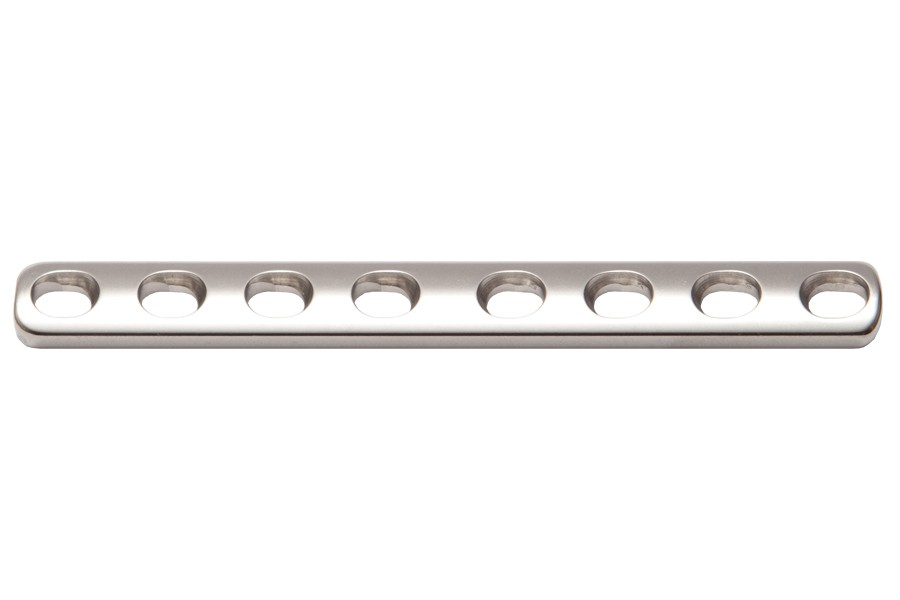
\includegraphics[width=12cm]{lcp.jpg}
\centering
\caption{Placa de compresión de bloqueo, tomado de [].}
\label{im5}
\end{figure}
\medskip

De igual forma, dentro del sector cultural,se ha trabajado en la caracterización de artefactos arqueológicos, con el fin de preservar la memoria cultural colectiva de la sociedad se deben crear bases de datos digitales donde se guarden digitalizaciones tridimensionales de estos objetos debido a que muchas veces estos objetos terminan deteriorándose por el paso del tiempo, desastres naturales, o por la acción del hombre.
%
La investigación del grupo ha estado orientada a digitalización tridimensional a través del sensor Kinect. Sin embargo no se ha encontrado una resolución del método muy alta; el método de proyección de franjas puede responder a esta necesidad, más exactamente, el presente trabajo puede responder a esta necesidad, dado que muchos de estos objetos pueden presentar alta reflectividad.
%

\begin{figure}[h!]
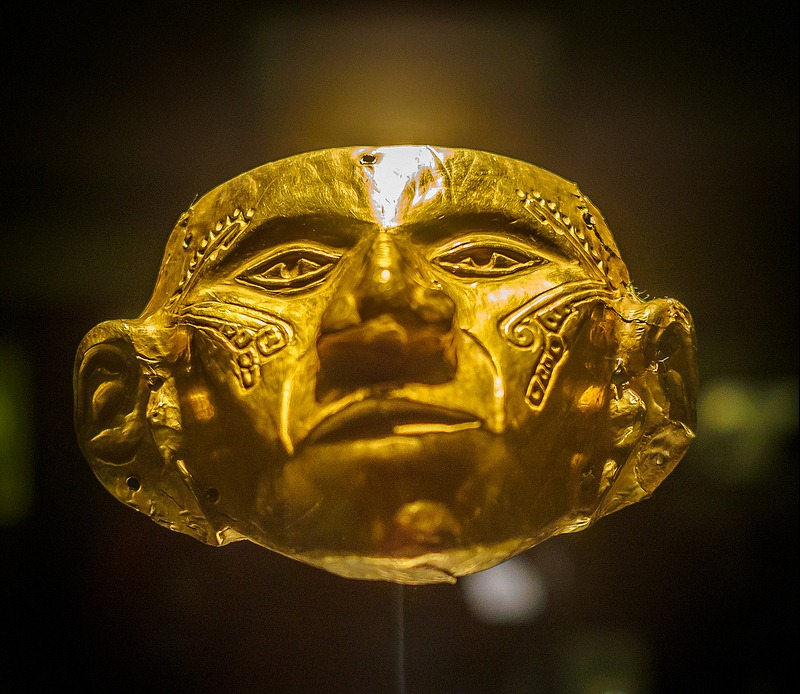
\includegraphics[width=9cm]{Goldenmask.jpg}
\centering
\caption{Máscara de oro del museo del oro, Bogotá, Colombia, tomado de [], ejemplo de un artefacto arqueológico con alta reflectividad.}
\label{im5}
\end{figure}
\medskip


%el sector industrial y médico [] requieren poder caracterizar y realizar control de calidad a productos metálicos, que tienen alto reflectividad , así como el sector cultural [] , dado que objetos arqueológicos que se quieren digitalizar en bancos de datos también pueden estar hechos de materiales que tengan este problema.


%********************************** % Third Section  *************************************
\section{Objetivos}  %Section - 1.3 
%\label{section1.3}

\subsection{Objetivo principal}

%
Implementar una metodología en la digitalización tridimensional por proyección de franjas que permita su uso en objetos con alta reflectividad en su superficie.
\medskip

\subsection{Objetivos especificos} 

\begin{itemize}
\item Calibrar el sistema CCD-Objeto-Proyector.
\item Implementar ambos métodos para recuperar la fase en diferentes objetos con alta reflectividad.
\item Realizar una retroalimentación de los resultados en las digitalizaciones.
\end{itemize}





%\section{Desafío experimental}

%Muy a menudo al adoptar metodologías ajenas o al emplear objetos más exigentes que los usados en los estudios en los cuales se basa este proyecto de investigación se presentan problemas que deben ser abordados usando conocimiento empírico, intuición, o nuevas ideas, se declara como valor agregado de este proyecto que éste está sujeto a modificaciones que surjan para superar problemas en la fase de ejecución, y que, en primera medida, buscarán ser resueltos por el autor de este proyecto.

\section{Metodología}



\section{Cronograma}

\begin{table}[h]
\begin{center}
\begin{tabular}{|c|c|c|}
\hline
fase&Paso&Fecha\\
\hline
Preliminar&1& \\
\hline
Primera&2& \\
\hline
Segunda&3& \\
\hline
\end{tabular}
\end{center}
\end{table}







\end{document}